%\begin{savequote}[8cm]
%Alles Gescheite ist schon gedacht worden.\\
%Man muss nur versuchen, es noch einmal zu denken.

%All intelligent thoughts have already been thought;\\
%what is necessary is only to try to think them again.
 % \qauthor{--- Johann Wolfgang von Goethe \cite{von_goethe_wilhelm_1829}}
%\end{savequote}

\chapter{\label{ch-theory}Theory}

\minitoc

\section{Introduction}

\section{Plasmas and laser-plasma interactions}
\section{Hydrodynamics and the operation of hydrocodes}
\section{Key physics of ICF}
\section{Shocks and the Rankine-Hugoniot relations}

\subsection{Shocks physics}

Shocks, referring to a sudden change in plasma properties over a thin transition region, are ubiquitous in plasmas and inertial confinement fusion, occurring whenever there is a change in the pressure applied to the capsule. Generating and measuring the plasma state produced by a shock was also the key feature of the experiment described in \hl{SECTION}. As such, this section will provide a brief overview of the key principles of shock physics, based on the explanation in \cite{Zeldovich1966}.

\begin{figure}
\centering
\includegraphics[width=0.6\textwidth]{figures/Theory/Piston.pdf}% Here is how to import EPS art
\caption{\label{fig:Piston} A piston, moving at velocity $u$ drives a shock through a medium. The shock moves at velocity $D$, leaving material behind it in a new shock state denoted by the subscript 1. Based on a diagram in \cite{Zeldovich1966}.}
\end{figure}

Consider the situation in Figure \ref{fig:Piston}. The material is initially at rest, until it is disturbed by a piston moving at velocity $u$, and applying a pressure $P$. After a time $t$, the piston has moved by a distance $ut$. This drives a disturbance (shock) through the material with a velocity $D$, which is now at the position $Dt$. Behind the shock the material is at the piston pressure and velocity $P$ and $u$, and at a new higher density $\rho_1$. Ahead of the disturbance, the material is unaffected.

Three equations can be derived based on the conservation of mass, momentum, and energy across the disturbance. Considering that the mass in distance $DT$ cannot have changed, the expression
\begin{equation} \rho_0 D = \rho_1 (D-u) \end{equation}
is obtained. (Here, as in the following equations, $t$ and the area $A$ cancel from both sides of the equation. Considering the momentum of this material (which changes according to the impulse, arising from the difference in pressure either side of the boundary), leads to the equation 
\begin{equation} \rho_0 D u = P_1 - P_0. \end{equation}
Finally, considering the change in total energy (both internal energy $\epsilon$ and kinetic energy), which must equal the work applied by the piston as it moves the distance $ut$, results in the third equation 
\begin{equation} \rho_0 D (\epsilon_1 - \epsilon_0 + \frac{u^2}{2}) = P_1 u. \end{equation}

These equations relate the four shock variables $D$,$u$,$P$ and $\epsilon$ to one another. If the state of the material ahead of the shock is known, then finding any two of these variables allows the other to be calculated. They are referred to collectively as the Rankine-Hugoniot relations. They were derived here in a stationary frame (where the shock moves with velocity $D$), and are typically expressed as
\begin{equation} \rho_1 = \frac{\rho_0 D}{D - u}, \label{eqn: RH1 stationary} \end{equation}
\begin{equation} P_1 - P_0 = \rho_0 D u, \label{eqn: RH2 stationary} \end{equation}
\begin{equation} \epsilon_1 - \epsilon_0 = \frac{P_1 u}{\rho_0 D} - \frac{u^2}{2}. \label{eqn: RH3 stationary} \end{equation}

\subsection{Rankine-Hugoniot relations in a moving frame}

\begin{figure}
\centering
\includegraphics[width=0.8\textwidth]{figures/Theory/ReferenceFrames.pdf}% Here is how to import EPS art
\caption{\label{fig:ReferenceFrames} The shock as viewed in the two frames. In the stationary frame, the shock moves with velocity $D$, the shocked material with velocity $u$, and the unshocked material is stationary. In the moving frame, the shock is stationary, the shocked material has velocity $u_1$, and the unshocked material has velocity $u_0$. The other variables are unchanged.}
\end{figure}

Alternatively, the same equations can be considered in a moving frame, where the shock is stationary. The frame now moves at velocity $D$, as displayed in Figure \ref{fig:ReferenceFrames}. This means the unshocked material moves into the stationary shock front at a velocity $u_0 = -D$, while the material behind the shock moves away at the slower velocity $U_1 = -(D - u)$. This transformation can be applied to each of Equations \label{eqn: RH1 stationary}, \label{eqn: RH2 stationary} and \label{eqn: RH3 stationary} to give the Rankine-Hugoniot relations in an alternative form,
\begin{equation} \rho_1 u_1 = \rho_0 u_0, \label{eqn: RH1 moving} \end{equation}
\begin{equation} P_1 + \rho_1 u_1^2 = P_0 + \rho_0 u_0^2, \label{eqn: RH2 moving} \end{equation}
\begin{equation} \epsilon_1 + \frac{P_1}{\rho_1} + \frac{u_1^2}{2} = \epsilon_0 + \frac{P_0}{\rho_0} + \frac{u_0^2}{2}. \label{eqn: RH3 moving} \end{equation}
These three relations can also be derived by integrating over the differential equations describing the conservation equations given in \hl{SECTION}.

These equations can be further manipulated to derive some other useful expressions. Equations \ref{eqn: RH1 moving} and \ref{eqn: RH2 moving} can be used to find new expressions for the velocities $u_1$ and $u_0$, 
\begin{equation} u_1^2 = \nu_1^2 \frac{P_1 - P_0}{\nu_0 - \nu_1}, \label{eqn: RH moving u1} \end{equation}
\begin{equation} u_0^2 = \nu_0^2 \frac{P_1 - P_0}{\nu_0 - \nu_1}, \label{eqn: RH moving u0} \end{equation}
where $\nu$ is the specific volume, $\nu = \frac{1}{\rho}$. Substituting Equations \ref{eqn: RH moving u1} and \ref{eqn: RH moving u0} into Equation \ref{eqn: RH3 moving} then gives
\begin{equation} \epsilon_1 - \epsilon_0 = \frac{1}{2}(P_0 + P_1)(\nu_0 - \nu_1).\label{eqn: Hugoniot relation} \end{equation}

Equation \ref{eqn: Hugoniot relation} is known as the Hugoniot relation. The Hugoniot curve can also be defined, 
\begin{equation} P_1 = H(P_0, \nu_0, \nu_1),\label{eqn: Hugoniot relation} \end{equation}
which has a form which depends on that of the specific energy function $\epsilon(P, \nu)$. The form of the Hugoniot curve is notable as it is a function of two parameters - the initial state of the material $(P_0, \nu_0)$. The significance of this will be discussed in the next section.

\subsection{The Hugoniot}

The Hugoniot curve describes the locus of possible shock states that can be achieved when a single shock is driven through a target with the specified initial state. It is formally defined as a function of $P$ and $\nu$ but the Rankine-Hugoniot relations mean it can be equivalently expressed as a function of any two of the shock variables, and it is often more convenient to discuss it in $(P, \rho)$ or $(P, u)$ space. Discussion of the Hugoniot and this topic can be found in \cite{Forbes2012}.

\begin{figure}
\centering
\includegraphics[width=0.8\textwidth]{figures/Theory/SecondaryHugoniot.pdf}% Here is how to import EPS art
\caption{\label{fig:SecondaryHugoniot} a) The principal Hugoniot in $(P, \rho)$ space. A shock compresses material in the intial state along a compression path described by the Rayleigh line to a shock state on the Hugoniot curve. The curve represents the range of possible shock states that could be achieved for a given initial state. b) If a subsequent shock passes through the material, the shock state it will generate lies somewhere on a secondary Hugoniot, which is a unique curve generated for the new initial condition (the shock state achieved by the first shock).}
\end{figure}

The dependence of the Hugoniot on the initial state is significant, as is highlighted in Figure \ref{fig:SecondaryHugoniot}. For the initial state $(P_0, u_0)$, the Hugoniot curve is plotted; this describes the states accessible by a shock from that initial point. Driving a shock with pressure $P_1$ through the target allows the shock state $(P_1, u_1)$ to be achieved. However, following this with a higher shock does not allow a new state on this curve to be accessed, due to the fact that the material ahead of this new shock is no longer $(P_0, u_0)$, is but instead $(P_1, u_1)$. To find the state achieved by this second shock requires a new Hugoniot curve to be plotted, $P_2 = H(P_1, \nu_1, \nu_2)$; this curve will pass through the state $(P_1, u_1)$, and describe the locus of states that the new shock can reach.

The Hugoniot curve describing the states that can be accessed from an initially unshocked material, $P_1 = H(P_0 = 0, \nu_0, \nu_0)$, is particularly significant for two obvious reasons; most materials begin experiments unshocked (and so the first shock state achieved will be on this curve), and the states on this curve are the easiest to measure and access. This curve is known as the `Principal Hugoniot'. This curve can be populated experimentally by measuring the state achieved when shocks of different strengths are passed through initially unshocked material.

It is also worth noting that the Hugoniot curve is not the path that the material takes through $(P, \nu)$ space as it is compressed (rather, it is the possible end states of such a compression). The the compression path is given by a different curve called the `Rayleigh line' \cite{Forbes2012}. The Rayleigh line is described by Equation \ref{eqn: RH2 stationary}, repeated below:
\begin{equation} P_1 - P_0 = \rho_0 D u.  \end{equation}
Note here that in $(P, u)$ space, the Rayleigh line in a straight line with a gradient of $Z = \rho_0 D$. If a shock travels through the material with a shock velocity $D$, then the final shock state will be the intercept between the Rayleigh line and the Hugoniot. This gradient $Z$ is called the shock impedance , and is significant when considering shocks between different materials. 

\subsection{Material interfaces and impedance matching}

The previous sections have considered shocks moving through a single material - material interfaces will now be considered. This section follows the descriptions given in \cite{Forbes2012} and \cite{Davison2008}. Imagine a shock $S_1$ travelling through material A, which then reaches an interface with material B. Some fraction of the shock energy will be transmitted across the interface into material B, while some will be reflected into material A. The pressure behind the reflected shock $P_R$ is given \cite{Colvin2013} by 
\begin{equation} \frac{P_R}{P_1} = \frac{Z_2 - Z_1}{Z_2 + Z_1}.  \end{equation}
Three illustrative cases are useful to consider. If the impedances of the two materials are very similar $Z_2 \approx Z_1$, the reflected shock pressure will be effectively zero and almost all the shock energy propagates into the new material. If there is a high impedance mismatch between the materials, then a large fraction of the shock energy is reflected. If the new material is higher impedance $Z_2 > Z_1$, then the reflected pressure is positive and a shock is reflected. If the new material is instead low impedance $Z_2 < Z_1$ then the rarefaction/relaxation wave is instead reflected.

The state achieved either side of the interface after the shock crosses it can be found through an impedance matching calculation. This relies on a key principal. After the shock has crossed the interface, the material on either side is in the state achieved by the transmitted/reflected waves $S_2$ and $S_3$. For the two materials to remain in contact, it is required that the pressure $P$ and particle velocity $u$ of the material either side of the boundary must be equal - if this were not the case, the boundary would not be in equilibrium, or the two layers would separate. This enables impedance matching calculations, where the state in each material following the shock crossing the interface can be determined.

\begin{figure}
\centering     %%% not \center
\subfigure{a)\includegraphics[width=.45\textwidth]{figures/Theory/ShockDiagram.pdf}}
\subfigure{b)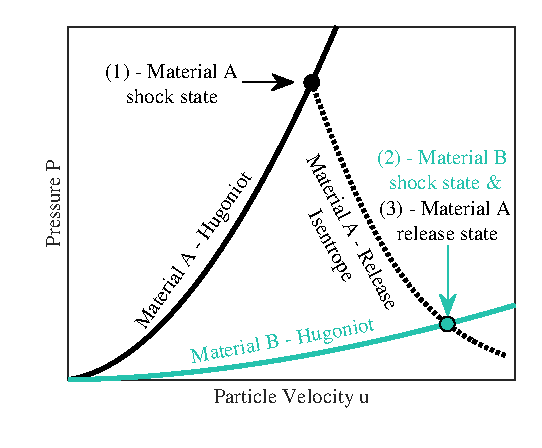
\includegraphics[width=.45\textwidth]{figures/Theory/MatlabIM1.eps}}
\caption{ \label{fig:ShockDiagramAndIMTheory1} a) x-t diagram showing a shock transiting across the interface from a high impedance material into a low one. The dashed line shows the material interface, while the arrows show the shocks. The shock/rarefaction waves are refered to as $S_n$, while the shock states are refered to by the numbers. b) $(P,u)$ plot showing the impedance matching graphically. $S_1$ shocks material in state (0) to a state (1) on the Hugoniot for quartz A. Rarefaction wave $S_3$ causes A to relax from (1) to a state (3 on the release isentrope for A. Shock $S_2$ shocks B from state (0') to state (2) on the foam Hugoniot. The impedance matching criteria means that (2) and (3) are equivalent in $(P,u)$ space, and thus this state is found as the intercept of these two curves.}
\end{figure}

This is shown graphically for the case where the second material is lower impedance in Figure \ref{fig:ShockDiagramAndIMTheory1}. The shock initially travels through material A, where it sees the unshocked material. It therefore leaves this material in the state $(P_1, u_1)$, which lies on the Principal Hugoniot for the material. The shock reaches the interface, and generates a rarefaction wave $S_2$ which travels back into material A, and a shock wave $S_3$ which propagates through material B. As material B is unshocked, the new state $(P_3, u_3)$ lies on the Principal Hugoniot for that material. Rarefaction wave $S_2$ travels through the pre-shocked state $(P_1, u_1)$, and causes it to relax to a new state $(P_2, u_2)$. This relaxation occurs along another curve known as the release isentrope, which describes the locus of states that the material could relax to given it's shocked initial state of $(P_1, u_1)$. As impedance matching requires that the pressure and particle velocity must be constant across the interface after the shock has transited, it is clear that such that $P_3 = P_2$ and $u_3 = u_2$. There will be a single $(P, u)$ state which lies on both the release isentrope and hugoniot, which defines the state in both materials\footnote{There are two things to note here. 1) There is only one state which satisfies this condition. However, if the shock $S_1$ strength is changed, the state $(P_1, u_1)$ is changed, and thus the release isentrope (which depends on this initial state) also changes - meaning that the impedance matching criteria where the Hugoniot B and release isentrope are satisfied now also occurs at a different point. 2) While the $(P,u)$ state of the two materials is equivalent, the Rankine-Hugoniot equations used to calculate the other variables reference the initial state of the material being considered - meaning that the other shock variables for these materials will not be equal.}.

The case when the new material is higher impedance is similar, but with a few key differences. In this case the new pressure $P_3 = P_2$ is greater than the original pressure $P_1$. The wave $S_2$ which reflects from the interface back into material A is now no longer a rarefaction wave, but another shock. This means that the new state is a state on the shock Hugoniot for A with initial conditions $(P_1, u_1)$, rather than a state on the release isentrope. However, the impedance matching condition $P_3 = P_2$ and $u_3 = u_2$ still applies, and thus in this case it is the principal Hugoniot of A and the secondary Hugoniot of B which are found to overlap.

\subsection{Measuring shock states experimentally}

%It was shown earlier in this section that the Rankine-Hugoniot relations allow all the shock variables associated with a shock state to be calculated, if at least two of the variables (and the state of the unshocked material) are already known. Experiments to measure shock states therefore require the measurement of any two of these variables. `Absolute' shock state measurements measure two such variables directly. 

%However, impedance matching provides a way to determine the shock state of a material by only measuring one of these variables directly. This relies on the situation described in the previous subsection. A known reference material, which is already well-characterised, is placed in contact with the material of study. Aluminium or quartz are typical examples. A shock is then driven through the reference material, such that it crosses the interface into the material being studied. As discussed, this will result in a shock/rarefaction (depending on the relative impedance) wave propagating back into the reference, and the pressure and particle velocity in the reshocked/relaxed reference and the shocked material of study will be equal.

%This is performed in such a way that the shock velocity can be measured in both materials. The shock velocity in the reference material during the first shock is measured, and this is used to plot the Rayleigh line $P_1 = \rho_0 D u$ in the reference. The intercept of the Rayleigh line and the Hugoniot defines the shock state that the reference material reaches after the first shot. When the reflected shock/rarefaction wave propagates back through the reference, this material will be shocked/relaxed according to an as yet undetermined point somewhere on the known reference Hugoniot/release isentrope. 

%Following the theory in the previous section, it is clear the 

It was shown earlier in this section that the Rankine-Hugoniot relations allow all the shock variables associated with a shock state to be calculated, if at least two of the variables (and the state of the unshocked material) are already known. Experiments to measure shock states therefore require the measurement of any two of these variables. `Absolute' shock state measurements measure two such variables directly. However, impedance matching can be used to enable the determination of a new shock state by instead measuring only one variable - the shock velocity - in two different materials, which can be simpler experimentally.

\begin{figure}
\centering
\includegraphics[width=0.6\textwidth]{figures/Theory/MatlabIM2.eps}% Here is how to import EPS art
\caption{\label{fig:IMTheory2} A $(P,u)$ plot as in Figure \ref{fig:ShockDiagramAndIMTheory1}, showing how impedance matching is used experimentally. Material A is a reference, where the Hugoniot and release isentrope are known. Measuring the shock velocity of $S_1$ in A allows the Rayleigh line to be plotted - the intercept of this with the known Hugoniot for A allows state (1) to be determined. Measuring the shock velocity of $S_2$ in B also allows a Rayleigh line to be plotted for this shock. The intercept of this line with the known release isentrope A allows the state (2), a shock state of B which lies on the unknown Hugoniot of B, to be calculated.}
\end{figure}

Consider the situation described in the previous section, where material A is a known reference (which means that the relevant curves, such as the Hugoniots and the release isentrope, are already known) and material B is the material of study. Imagine that this scenario is set up so that the shock velocities corresponding to the original shock in the reference material $S_1$ and the new shock $S_2$ are measured.

Measuring the shock velocity $U_{S_1}$ allows the Rayleigh line for this shock to be plotted, and the intercept of this curve with the known principal Hugoniot of the reference is the initial shock state achieved in this material $(P_1, u_1)$. This is shown in Figure \ref{fig:IMTheory2}. This is then used to calculate the relevant secondary Hugoniot or release isentrope for the reference (the choice of curve depends on the impedance). Measuring the shock velocity $U_{S_2}$ enables the Rayleigh line for the transmitted shock to be plotted, and the intercept with the Hugoniot for material B would define the shock state for that material. The impedance matching criteria means that as this is the same $(P, u)$ state achieved in the reshocked/relaxed reference, this state also lies on the known secondary Hugoniot/release isentrope for the reference. The Hugoniot for the material of study is not known, but this shock state on it can therefore be identified from the intercept between the Rayleigh line and the reference Hugoniot/release isentrope. Thus, the shock state is identified only from measurements of the two shock velocities, and knowledge about the reference material.

\section{Equation of State and the principle Hugoniot}